\begin{figure}[t]
\centering
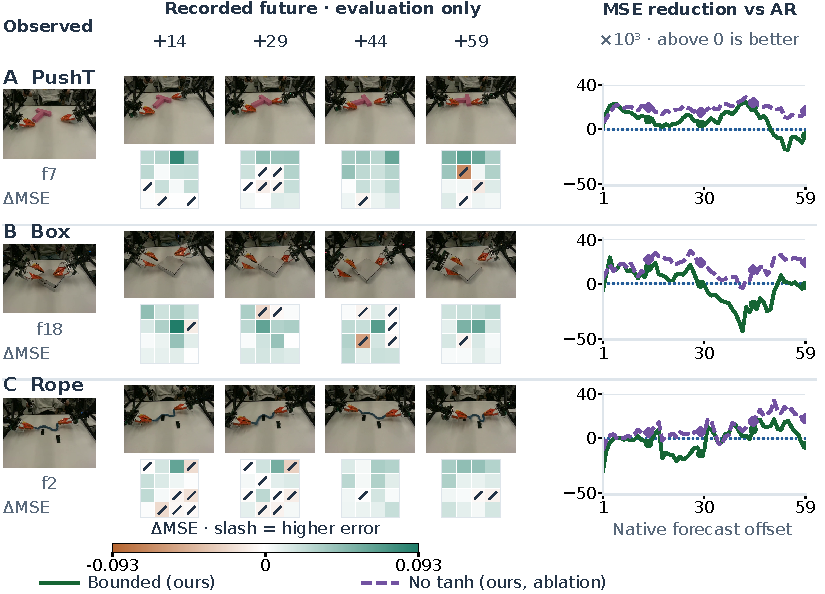
\includegraphics[width=\linewidth]{generated/qualitative_temporal_v1/temporal_outcomes.pdf}
\caption{\textbf{When and where do the forecasts differ?}
The same middle-ranked IWS windows as Figure~\ref{fig:closest-iws-gallery}
are followed across all 59 measured forecast offsets, without reselecting cases.
Left: the single observed frame. Center: recorded, withheld future frames at
offsets 14, 29, 44 and 59; these are evaluation context, not predicted RGB.
The aligned $4\!\times\!4$ maps show autoregressive minus no-$\tanh$ feature MSE:
teal is lower error for the ablation, brown and diagonal marks mean higher error, on one shared symmetric
scale. Right: the same error difference averaged over all patches, multiplied
by $10^3$, for bounded ShiftWM (solid) and no-$\tanh$ (dashed). Zero is the
matched autoregressive reference. All curves include their early and late
regressions; markers identify the four mapped offsets. Values average three
seeds after computing squared errors. Each task uses its own training-only
standardization; shared scales do not compare task difficulty. The patch features are contextual, so
these maps are not pixel-error localization or semantic attention.
Recorded scenes: RLA-WM/IWS dataset.}
\label{fig:temporal-qualitative-outcomes}
\end{figure}
